\documentclass[11pt]{article}

\usepackage{graphicx} % for inputing graphics
\usepackage{epstopdf} % Helper Package to graphix package
\usepackage{fancyvrb} % for \VerbatimInput (the nice inline code refrences)
\usepackage{amssymb} % American Math Society package, creates theorems and more math things 
\usepackage{caption} %creates captions for figures and other floating objects in paper 
\usepackage[fleqn]{amsmath} %flegn- moves equations to the left amsmath-helps with equation building other math things
\usepackage{tipa} % imports greek characters and other random letters heres a cool cheat sheet! https://ptmartins.info/tex/tipacheatsheet.pdf
\usepackage{tipx} % additional font comands for the tipa package. not 100%
\usepackage{breakcites} % an asthetics feather that makes a line break after citations 
\usepackage{makeidx}
\usepackage[hyperpageref]{backref}

\usepackage{color}
\definecolor{MyDarkGreen}{rgb}{0.0,0.4,0.0}
\definecolor{MyDarkRed}{rgb}{0.4,0.0,0.0} 
\definecolor{MyBlue}{rgb}{0.0, 0.0, 0.5} 
\definecolor{MyOrange1}{rgb}{1.0, 0.9, 0.0} 

\usepackage[colorlinks=true, urlcolor= MyBlue, linkcolor= MyBlue, citecolor=MyDarkGreen ]{hyperref}

\setcounter{secnumdepth}{3}
\setcounter{tocdepth}{3}
\makeindex

\DeclareCaptionLabelSeparator{space}

\DeclareGraphicsRule{.tif}{png}{.png}{`convert #1 `dirname #1`/`basename #1 .tif`.png}
\textwidth = 6.5 in
\textheight = 8.2 in
\oddsidemargin = 0.0 in
\evensidemargin = 0.0 in
\topmargin = 0.0 in
\headheight = 0.0 in
\headsep = 0.7 in
\parskip = 0.2in
\parindent = 0.0in

% defining thorems corollarys and definitions 
\newtheorem{theorem}{Theorem}
\newtheorem{corollary}[theorem]{Corollary}
\newtheorem{definition}{Definition}

\setlength{\parindent}{1cm}
\newcommand{\abstractinenglishname}{Abstract}
\newenvironment{abstractinenglish}{
        \def\abstractname{\abstractinenglishname}
	\begin{abstract}
}{
        \end{abstract}
}

%title, author, date defineing
\title {Which Modern-Day Music Artist is William Shakespeare Most Similar to\\[1ex]}
\author{
Angel Sierra, 
Dominique McDonald,
Mariana Gonzalez Castro, \\
Danny Ying,
and Carina Kalaydjian \\[1ex]
}
\date{June 7th, 2022}
%%%%%%%%%%%%%%%%%
%	HELPFUL BIBLIOGRAPHY KEY
% Here im going to list all the bibliography entries refnrece names and a short description of what the refrence is refrencing. 
% This way, all the refrences are here and no need to look back and forth to the bib file to cite stuff
%
% example: \cite{monkey} will cite "what is tech analysis a begginers guide", from monkeylearn.com
%
% refrence name - description
% monkey - what is tech analysis a begginers guide, monkeylearn.com
% web1 - Natural Language Processing with R,  Udacity.com  
% web2 - text mining and sentiment analysis: analysis with R, red-gate.com
% briney2015data - the briney book from class? i added it but not sure if we will need it 
% syuzhet - syuzhet package documentation in R 
% sonnetsData - refrences all of shakespears sonnets from the gutenberg project
% musicData - Refrences kaggle dataset with the music artists and their lyrics
% tm - Tm: text mining package documentation in R
% shakeFacts - fun facts about william shakespear 
% scienceDirect - Chapter 4: Text Mining and Network Analysis of Digital Libraries in R
% k-means - K-means Clustering: Algorithm, Applications, Evaluation Methods, and Drawbacks, from towardsdatascince.com
% NLP-for-music - Natural language processing for music knowledge discovery, article 
% NLP-for-lyrics - Natural language processing of lyrics, article
% knowledge-graphs - An Introduction to Knowledge Graphs, from standord AI labs 
% nrc-sentiment - NRC Word-Emotion Association Lexicon
%%%%%%%%%%%%%%%%%%

\begin{document}

\maketitle
\vspace{6pt}

\begin{abstractinenglish}
\emph{abstract text goes here here here here here here here here!!!!!!!!!!!!!!!!!!!!!!!!!!!!!!!}
\end{abstractinenglish}

\section{Introduction}

%%%%%%%% Remove tester before submitting 
here we cite \cite{web1} our glorius leader \cite{web2} yeah yeah cool cool \cite{briney2015data} and this too \cite{monkey} this as well \cite{sonnetsData} woohooo!!! \cite{musicData} and \cite{syuzhet} and \cite{tm} and \cite{shakeFacts} sdljdj \cite{k-means} , \cite{NLP-for-music} and  \cite{NLP-for-lyrics}, \cite{knowledge-graphs}, \cite{nrc-sentiment}
%%%%%%%%%%%%%%%%%%

\noindent  William Shakespeare is a world-renowned poet from 16th-century England. In his lifetime of 52 years, he wrote 37 plays, 154 sonnets, and many poems\cite{shakeFacts}. William Shakespeare has recognition for being one of the most revolutionary Literarry Artists to this date\cite{shakeFacts}. The Oxford Dictionary of Quotations states that William Shakespeare wrote close to one tenth of the most quoted lines ever written or spoken in English\cite{shakeFacts}. Shakespeare is also the second most quoted English writer after the writers of the bible\cite{shakeFacts}. Through his work, Shakespear introduced almost  3,000 words to the English language, these words can still be found in the Oxford English Dictionary today\cite{shakeFacts}! Shakespeare has an incredible ability to deeply express emotions through his work. Reders have been inspired and moved by his work for centuries. Shakespeare changed the world through his literary works. That is why William Shakespear is the best candidate to analyze and see how his Literary work compares to modern-day music artists song lyrics. 

\noindent For this project we will be analzing Shakespeare's words and usage of emotion from his 154 sonnets from the Gutenberg Project\cite{sonnetsData}. We will then compare these words and emotions to another dataset of 45 different modern-day music artists and their song lyrics\cite{musicData}. Our interest is seeing which music artists song lyrics are the most similar to Shakespeare's sonnets in the aspect of two categories, similarities words used and similarities in emotions expressed. Then we will see which modern-day music artist is the most similar to Willam Shakspare.  

\noindent In order to answer this question, we are going to use various methods of Text Analysis, analysis of unorganized text data\cite{monkey}. The different forms of Text Analysis that we will be using for this project are Sentiment Analysis and Keyword Extraction. Sentiment Analysis involves analyzing the text and being able to extract the different emotions the text is expressing\cite{monkey}. Keyword Extraction analyzes the text and identifies which words appear most frequently in the text, these words are called Keywords\cite{monkey}. The combination of these two methods will bring the result of which music artist is the most similar to shakespear in therms of types of words used and which music artist is the most similar to Shakespeare in terms of emotion expressed through words.  

\section{Methods}
There is a growing demand for the application of Natural Language Processing to drive music knowledge discovery \cite{NLP-for-lyrics}. Within song lyrics there is a wealth of information that can be used to gain insights about the song and its listeners. The workflow used to conduct NLP is outlined in Oramas et. Al \cite{NLP-for-music} as the following steps 1. Corpus creation (collection of separated documents), 2. Text mining (accessing desired info and eliminating the excess), 3. Information extraction (word frequency, collocation, word position, etc.), 4. Knowledge graph generation (a directed labeled graph in which we have associated domain specific meanings with nodes and edges \cite{knowledge-graphs}), 5. Sentiment Analysis (Identify feelings and emotions present in a text \cite{monkey}).
 
\noindent This NLP pipeline can be applied to music to provide recommendations on what songs a listener might like based on what they already listen to. \cite{NLP-for-lyrics} This information is gathered by performing what’s called a similarity search. Mahedero et al \cite{NLP-for-lyrics} conducts a similarity search for their project by first calculating a similarity measure. The similarity measure used is known as the Standard Cosine Distance (SCD). The calculations of the SCD are beyond the scope of this paper, but something to note is that the SCD relies on the Inverse Document Frequency as a way to measure the prevalence of words in a document and compare that to other documents. 

\noindent As previously stated, we relied on Natural Language Processing methods to calculate the similarity between Shakespeare and current artists with the hope of identifying a single artist whose work has similar themes as Shakespeare’s. Our pipeline was structured similarly to that proposed in \cite{NLP-for-music} with the main difference being that we do not rely on knowledge graph generation to store any information or display findings. The methods that were most useful for this research were keyword extraction and sentiment analysis. Both methods of analysis provided us with crucial insights, so the details of each seem pertinent to share. 

\subsection{Keyword Extraction}
Keyword extraction is largely aimed at identifying the most relevant words in different texts and utilizing those words to understand common theme or popular topics.\cite{monkey} We used the tm library in R to perform keyword extraction\cite{tm} on the sonnets. This process involves first prepping the text by removing unwanted punctuation or numbers, eliminating stop words, changing everything to lower case. These transformations are necessary because when working with strings, you not only have to be precise, but you also must be exact. The cleaning process sometimes includes stemming the words, but we opted not to do that. Once the text is clean the idea is to create a table containing each word used in the text and the frequency with which it is used. To identify the top ten key words we sorted the words in the matrix by their frequency. 
%%%%%%%%%%% keywords shakespears wordcloud 
\begin{center}
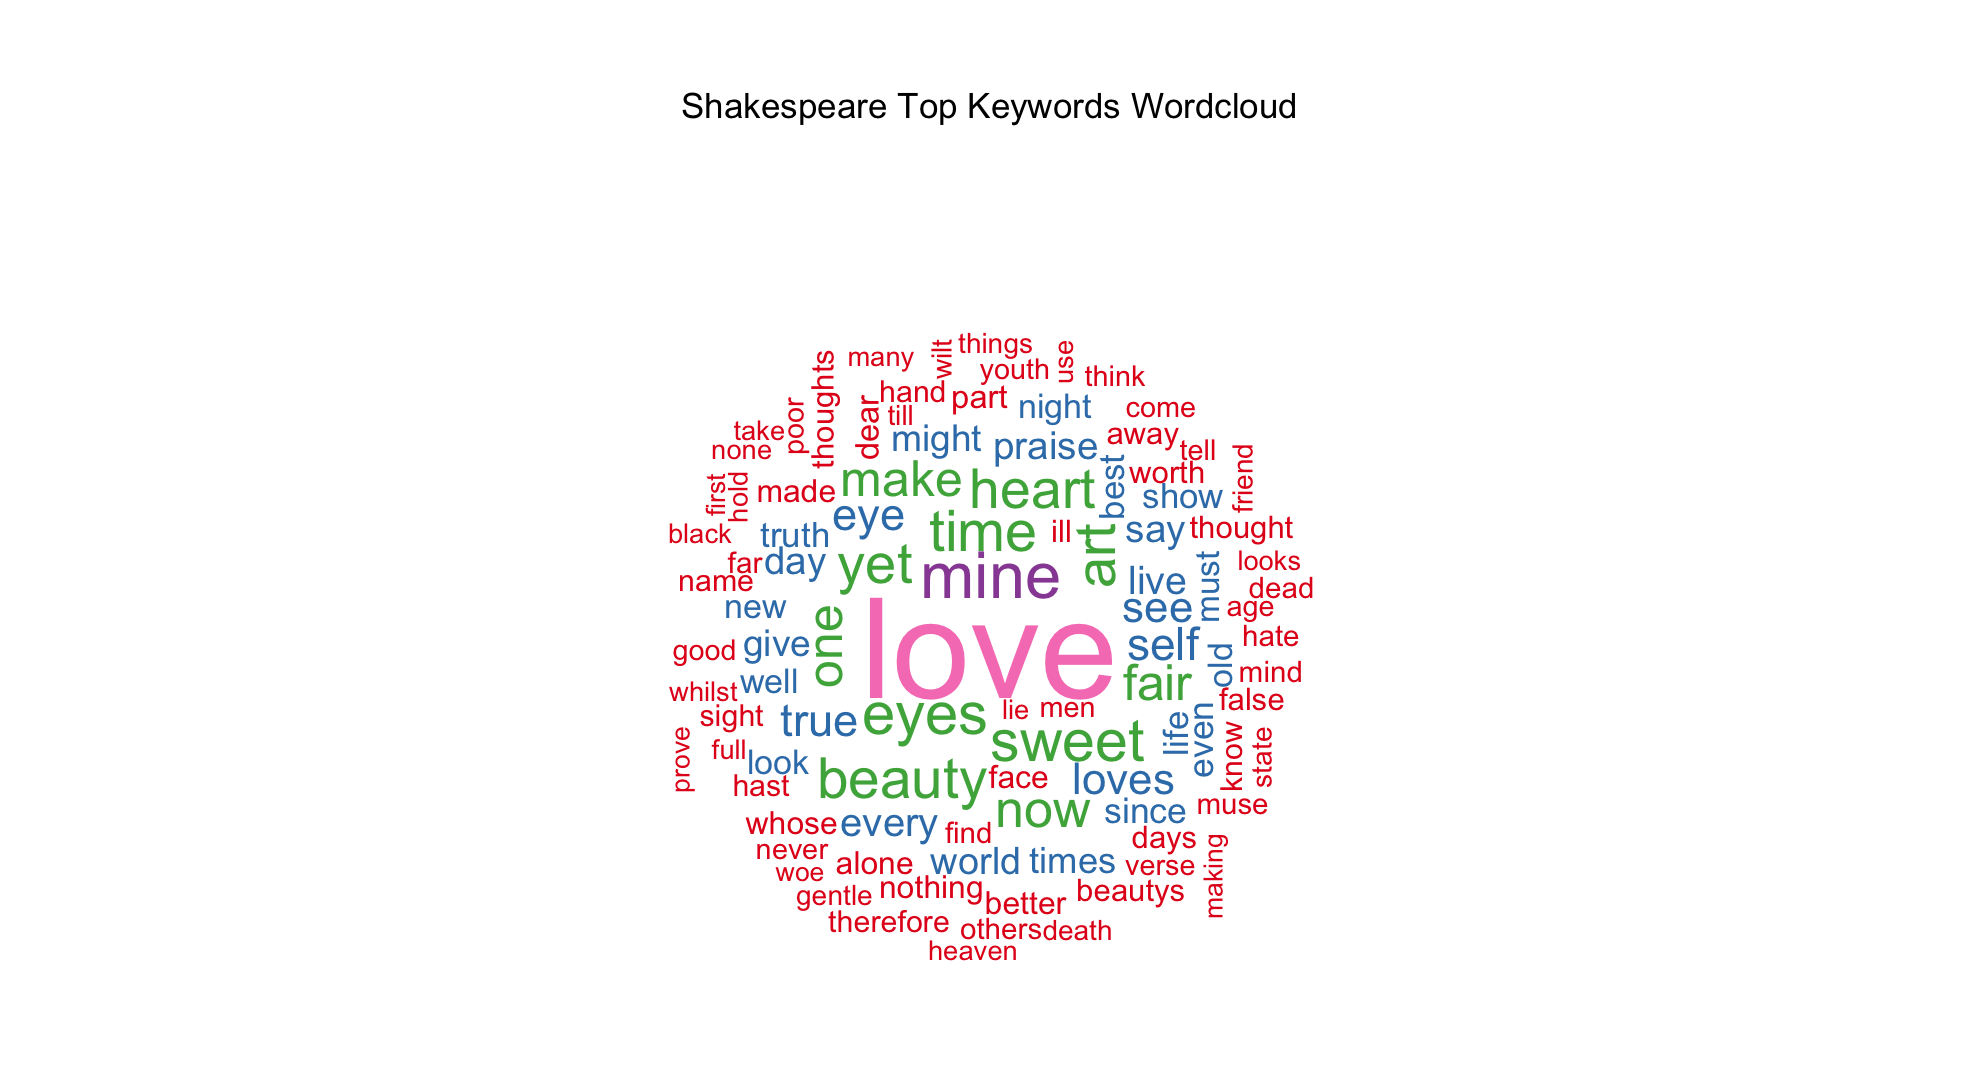
\includegraphics[width=14cm]{_assets/Shakespeare_Keywords_WordCloud.png}
\end{center}

\noindent Once Shakespeare’s keywords were identified, the next step was to identify the keywords for each of the 45 music artists. This process mirrored that of extracting keywords from the sonnets except we utilized an algorithm to automate the process for each artist. Once keywords were identified we converted the word frequencies for Shakespeare and all other artists into proportions, in order to standardize for comparison. To find the artists who were most like Shakespeare based on keywords, we checked for artist who had the highest number of matching keywords. Finally, then we ranked those by who used keywords in similar proportions to Shakespeare by calculating the Euclidian distance between the proportions of each of the matching keywords. This is similar to what Mahedero et. Al \cite{NLP-for-lyrics} does for their similarity search except we rely on word proportions and Euclidean distance, while their research utilizes Inverse Document Frequency and the Standard Cosine Distances. 

\subsection{Sentiment Analysis}
A similar sort of ranking was achieved from Sentiment Analysis, but the process has notable differences. The library syuzhet was used for the analysis. There is a wide variety of paths one could explore when performing sentiment analysis. Two that seemed viable for the purpose of this research were calculating an overall sentiment score and identifying the different emotions present in each text. \cite{syuzhet} The latter option proved to be more fruitful, as the analysis is more detailed. This process of classification based on emotion is known as NRC sentiment analysis. NRC Sentiment Analysis uses the National Research Council (NRC) Word-Emotion Association Lexicon to classify words in a text into eight categories of emotions. \cite{nrc-sentiment} It is important to note that a word may be associated with more than one emotion. The eight emotions are anger, anticipation, disgust, fear, joy, sadness, surprise, trust (include simple equation). \cite{nrc-sentiment} The objective of NRC Sentiment Analysis is to calculate the frequency with which each emotion is conveyed. This is calculated by identifying the emotions associated with the unique words in a text and summing up all the instances of each emotion\cite{syuzhet}. 

\noindent Once the NRC sentiments were calculated for both Shakespeare and the music artists, the frequencies were converted to proportions for accurate comparison. Using the proportions of each emotion, Euclidean distance was calculated for between each music artist and Shakespeare. The artists with the shortest distances from Shakespeare were considered the most similar to him, and therefore ranked higher in regard to comparison of the emotions conveyed in their works. 

\noindent After comparing results from each analysis method, a final ranking was calculated. This overall ranking was calculated by summing up the rankings from both analysis methods. Because similarity to Shakespeare was assessed using Euclidean distance, lower rankings signify higher similarity to Shakespeare. This meant that the artists with the lowest overall ranking mirrored Shakespeare’s work emotionally more than other artists.

\subsection{K-Means Clustering}
The NRC sentiments were utilized even further as predictors in K-Means Cluster Analysis. The objective of cluster analysis within the scope of this research is to utilize an unsupervised learning model \cite{k-means} to assess commonalities between the work of each music artist and Shakespeare. K-Means clustering is an iterative method that categorizes each data point into one of k predefined groups, or clusters. The process is driven by two objectives. The first being maximizing the distance between clusters, so that they are distinct. The second is minimizing the data points within a cluster, so the clusters themselves are homogenous. \cite{k-means} By employing K-means Clustering we were able to identify a group of artists that whose work most closely matches Shakespeare’s. 

%%%%%%%% (include cluster analysis plot)
\begin{center}

\includegraphics[width=14cm]{_assets/ClusterAnalysis_Fit10.png}
\end{center}

\subsection{Data Management}
Before discussing the results of our various methods, it is important to address what made such an undertaking possible: data management.  The size of this project necessitated multiple team members using multiple platforms. The data was stored in a relational database and then hosted on  Amazon Web Services(AWS) service called Relational Database Services(RDS). Using RDS preserves the database from alterations, each memeber each member provided the read only user credentials to their database to enable the team to access data without making changes to the database itself. Once we had the data it the next steps were to process and analyze it. 

\noindent Again, with so many contributors working to advance the project it was necessary to have an avenue for efficient and organized sharing of code. For this aspect of the project, GitHub was utilized and it allowed team members to work on the same files from different locations and share them as frequently as necessary. Along with our code we are also able to store and share important information that aided us in our research. The different information sharing structures employed allowed for efficient progression and ultimately valuable results. 






\section{Results}
%%%%%%%%%%%  sentiment analysis ranking table 
 \begin{table}[ht]
\centering
\begin{tabular}{lrr}
  \hline
Artist & Sent. Euclidean Distance & Sentiment Rank \\ 
  \hline
eminem & 0.00 &   1 \\ 
  nirvana & 0.00 &   2 \\ 
  cake & 0.00 &   3 \\ 
  amy-winehouse & 0.00 &   4 \\ 
  bob-dylan & 0.00 &   5 \\ 
  bob-marley & 0.00 &   6 \\ 
  johnny-cash & 0.00 &   7 \\ 
  nickelback & 0.00 &   8 \\ 
  britney-spears & 0.00 &   9 \\ 
  rihanna & 0.00 &  10 \\ 
   \hline
\end{tabular}
\caption{Ranked Top 10 Most Similar Music Artist to Shakespeare Based on Sentiments} 
\label{tab:wordranktable}
\end{table}

 
\newpage

%%%%%%%%%% all rankings table
\begin{table}[ht]
\centering
\begin{tabular}{lrrr}
  \hline
Artist & Word Rank & Sentiment Rank & Overall Rank \\ 
  \hline
amy-winehouse &   6 &   1 &   7 \\ 
  nickelback &   2 &   8 &  10 \\ 
  cake &   9 &   3 &  12 \\ 
  adele &   1 &  21 &  22 \\ 
  joni-mitchell &  11 &  11 &  22 \\ 
  leonard-cohen &   8 &  15 &  23 \\ 
  paul-simon &  10 &  22 &  32 \\ 
  blink-182 &  18 &  14 &  32 \\ 
  bob-marley &  27 &   6 &  33 \\ 
  rihanna &  25 &  10 &  35 \\ 
   \hline
\end{tabular}
\caption{Ranked Top 10 Most Similar Music Artist to Shakespeare} 
\label{tab:overallranktable}
\end{table}



%%%%%%%%%%%%%% include keyword rankings table here
\begin{table}[ht]
\centering
\begin{tabular}{lrrlr}
  \hline
Artist & Word Count & Frequency & Keyword & Word Rank \\ 
  \hline
adele &   3 & 626.00 &  love time heart &   1 \\ 
  nickelback &   3 & 11349.00 &  love time yet &   2 \\ 
  bieber &   2 & 648.00 &  love time &   3 \\ 
  dolly-parton &   2 & 685.00 &  love time &   4 \\ 
  dj-khaled &   2 & 928.00 &  mine time &   5 \\ 
  amy-winehouse &   2 & 3700.00 &  love time &   6 \\ 
  bjork &   2 & 5341.00 &  love yet &   7 \\ 
  leonard-cohen &   2 & 5972.00 &  love time &   8 \\ 
  cake &   2 & 7690.00 &  love time &   9 \\ 
  paul-simon &   2 & 8464.00 &  love time &  10 \\ 
   \hline
\end{tabular}
\caption{Ranked Top 10 Most Similar Music Artist to Shakespeare Based on Keywords} 
\label{tab:wordranktable}
\end{table}



% Example of how to refrence name of a code file in apendix 
% Examine and run \texttt{\char`_code\char`_A.R}
%
% Example of how to make latex print texts that looks like terminal commands 
% \begin{verbatim}
% install ccrypt
% \end{verbatim}

%example of how to insert a picture
%\begin{center}
%\includegraphics[width=14cm]{_assets/*some name*.png}
%\end{center}

\section{Conclusions}



\newpage
\section{Appendix}
Here's our code for the project
%\VerbatimInput{complete_analysis.R}

\newpage

\bibliographystyle{plain}
\bibliography{FinalArticle} 

\newpage{}
\include{appendicitis}




\end{document}